\chapter{Prototype/ Product Development}

\section{Introduction}

This chapter discusses the details of the prototype and product development concerning the Collective journaling application. It clarifies each interface of the mobile journaling system and provides additional information on front-end development using Flutter, back-end integration with Firebase, and AI-powered features through DeepSeek API. The chapter demonstrates how the prototype addresses the identified problems of digital journaling complexity while maintaining the intimate experience of traditional journaling.

\section{System Prototype}

The Collective journaling application is developed using Flutter framework with Dart programming language, providing cross-platform compatibility for both Android and iOS devices. Firebase serves as the backend-as-a-service platform, offering authentication, cloud storage, and real-time database capabilities. The system integrates with DeepSeek AI API for intelligent journal analysis and insight generation. Local storage is managed through Sembast database, ensuring offline functionality with automatic synchronization when connectivity is restored.

The application follows an offline-first architecture where users can write entries without internet connectivity, and the system automatically syncs data to the cloud when available. This approach addresses the core requirement of maintaining uninterrupted journaling experience regardless of connectivity status. The integration of Flutter, Firebase, and AI services ensures the system is both efficient and user-friendly while providing intelligent features that enhance the traditional journaling experience.

\section{Development Environment Setup}

The development environment utilizes Flutter SDK with the following key dependencies:
\begin{itemize}
    \item Flutter framework for cross-platform mobile development
    \item Firebase suite for authentication and cloud services
    \item Sembast for local database management
    \item HTTP client for DeepSeek API integration
    \item Material Design 3 for consistent UI components
    \item Camera and image processing capabilities for multimedia entries
\end{itemize}

The project structure follows Flutter best practices with organized directories for screens, services, models, widgets, and utilities. Custom plugins are maintained in the local\_plugins directory to address specific compatibility requirements, particularly for social authentication features.

\section{Collective Journaling Application Interface}

\subsection{Authentication System}

\subsubsection{Login Screen}

The login screen presents users with a clean, minimalist interface for accessing their existing accounts. The screen features the Collective logo and brand name prominently displayed at the top, establishing brand identity immediately upon app launch. Users can enter their email and password credentials in dedicated input fields with real-time validation feedback. The login form includes a "Forgot password?" link for password recovery and maintains consistent styling with rounded input fields and appropriate visual feedback for user interactions.

\begin{samepage}
\begin{figure}[H]
\centering

\includegraphics[width=0.35\textwidth]{files/imgs/prototype/auth_login.jpeg}
\caption{Login screen interface}
\label{fig:login-screen}
\end{figure}
\end{samepage}

\subsubsection{Registration Screen}

The registration screen expands the authentication interface to include additional fields for new user account creation. Users provide their first name, last name, email address, and password, with all fields featuring real-time validation to ensure data integrity and provide immediate feedback. The registration process includes email validation, password strength requirements, and clear visual indicators for required fields. Users can easily toggle between login and registration modes using the text link at the bottom of the screen.

\begin{samepage}
\begin{figure}[H]
\centering
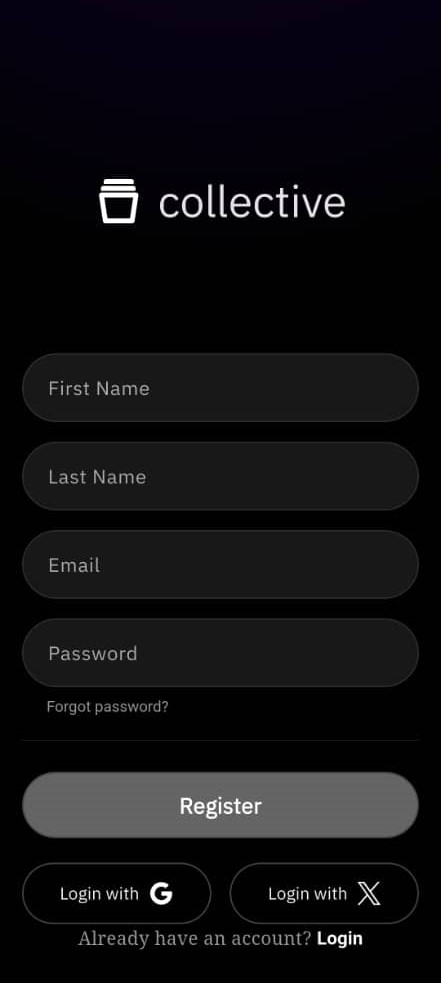
\includegraphics[width=0.35\textwidth]{files/imgs/prototype/auth_register.jpeg}
\caption{Registration screen with user details form}
\label{fig:registration-screen}
\end{figure}
\end{samepage}

\subsubsection{Google OAuth Integration}

The Google OAuth integration provides seamless authentication using existing Google accounts. The interface displays a dedicated button with the Google logo and clear labeling, allowing users to authenticate with a single tap without manual credential entry. The Google sign-in process leverages Firebase Authentication's OAuth provider, ensuring secure credential handling and automatic user profile creation upon successful authentication.

\subsubsection{Twitter/X OAuth Integration}

The Twitter/X OAuth integration offers an alternative social authentication method for users who prefer using their Twitter/X credentials. The interface includes a dedicated button with the Twitter/X logo, maintaining visual consistency with the Google OAuth option. The Twitter/X integration utilizes Firebase's OAuthProvider functionality with custom plugin modifications to ensure compatibility across different device configurations and handle edge cases in the authentication flow.

\begin{figure}[H]
\centering
\begin{minipage}{0.4\textwidth}
\centering
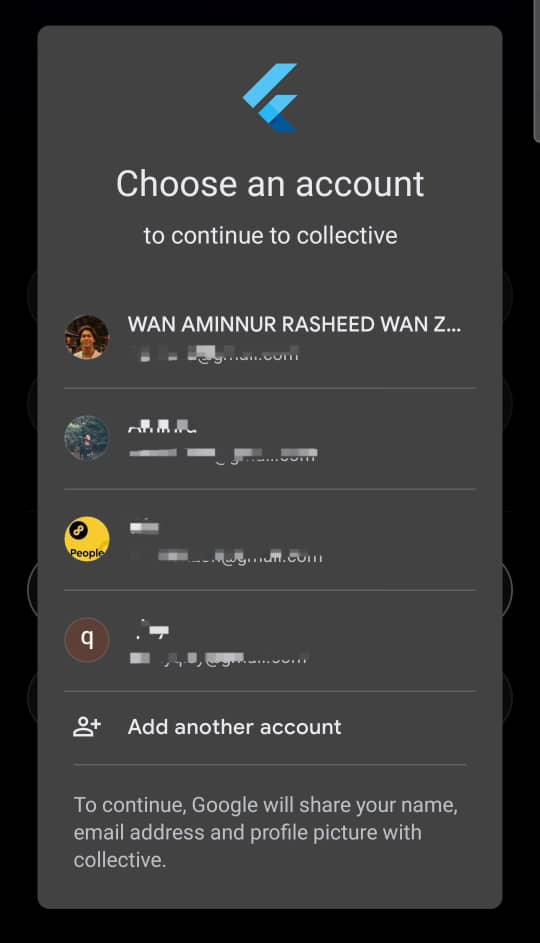
\includegraphics[width=0.8\textwidth]{files/imgs/prototype/google_oauth.jpeg}
\caption{Google and Twitter/X OAuth authentication}
\label{fig:google-oauth}
\end{minipage}
\hfill
\begin{minipage}{0.4\textwidth}
\centering
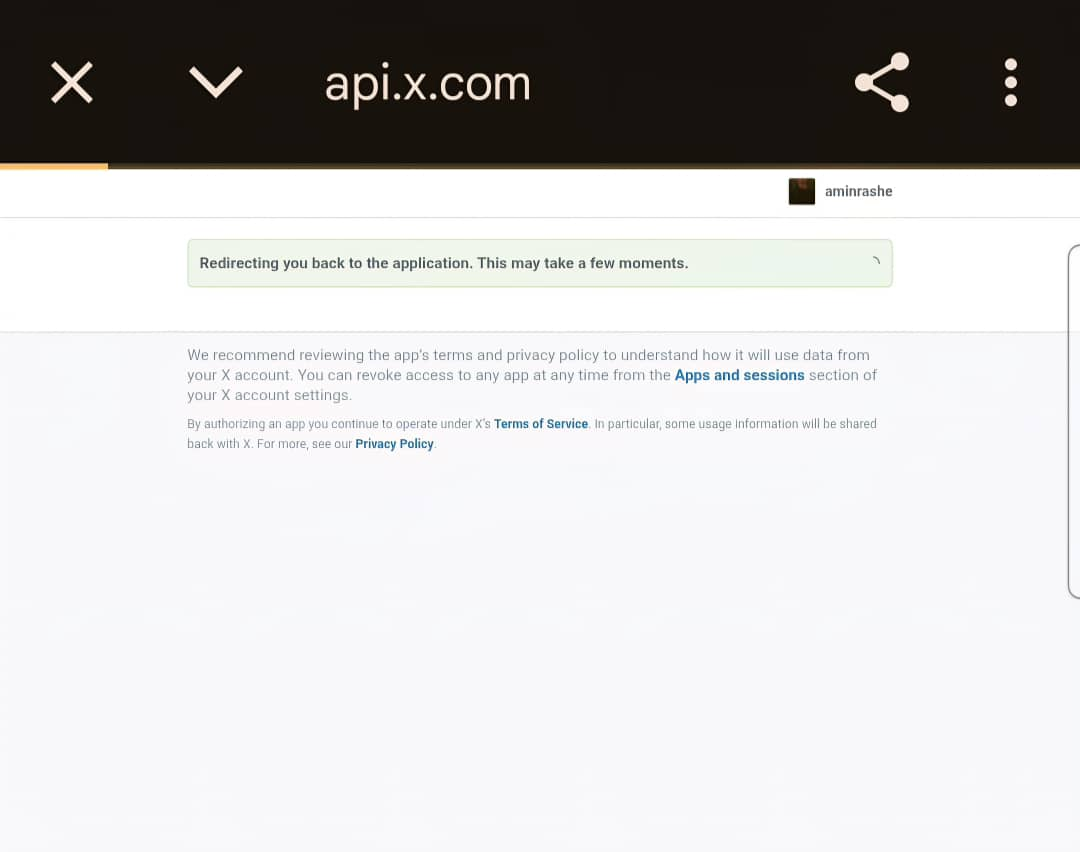
\includegraphics[width=0.8\textwidth]{files/imgs/prototype/x_oauth.jpeg}
%\caption{Twitter/X OAuth authentication}
\label{fig:twitter-oauth}
\end{minipage}
\end{figure}

\subsection{Main Journal Interface}

\subsubsection{Journal Home Screen}

The journal home screen represents the core interface where users interact with their entries. The design prioritizes content over navigation, featuring a clean timeline view of journal entries organized by date. Each entry is displayed as a card with the date, content preview, mood indicator, and associated tags. The interface includes a search functionality and selection mode for batch operations like favoriting or deleting entries. The screen includes a toolbar with options for creating new entries, searching through existing content, and accessing analytics. Entries are grouped by date with sticky headers for easy navigation. The interface supports infinite scrolling and includes loading states with shimmer effects for smooth user experience.

\begin{samepage}
\begin{figure}[H]
\centering
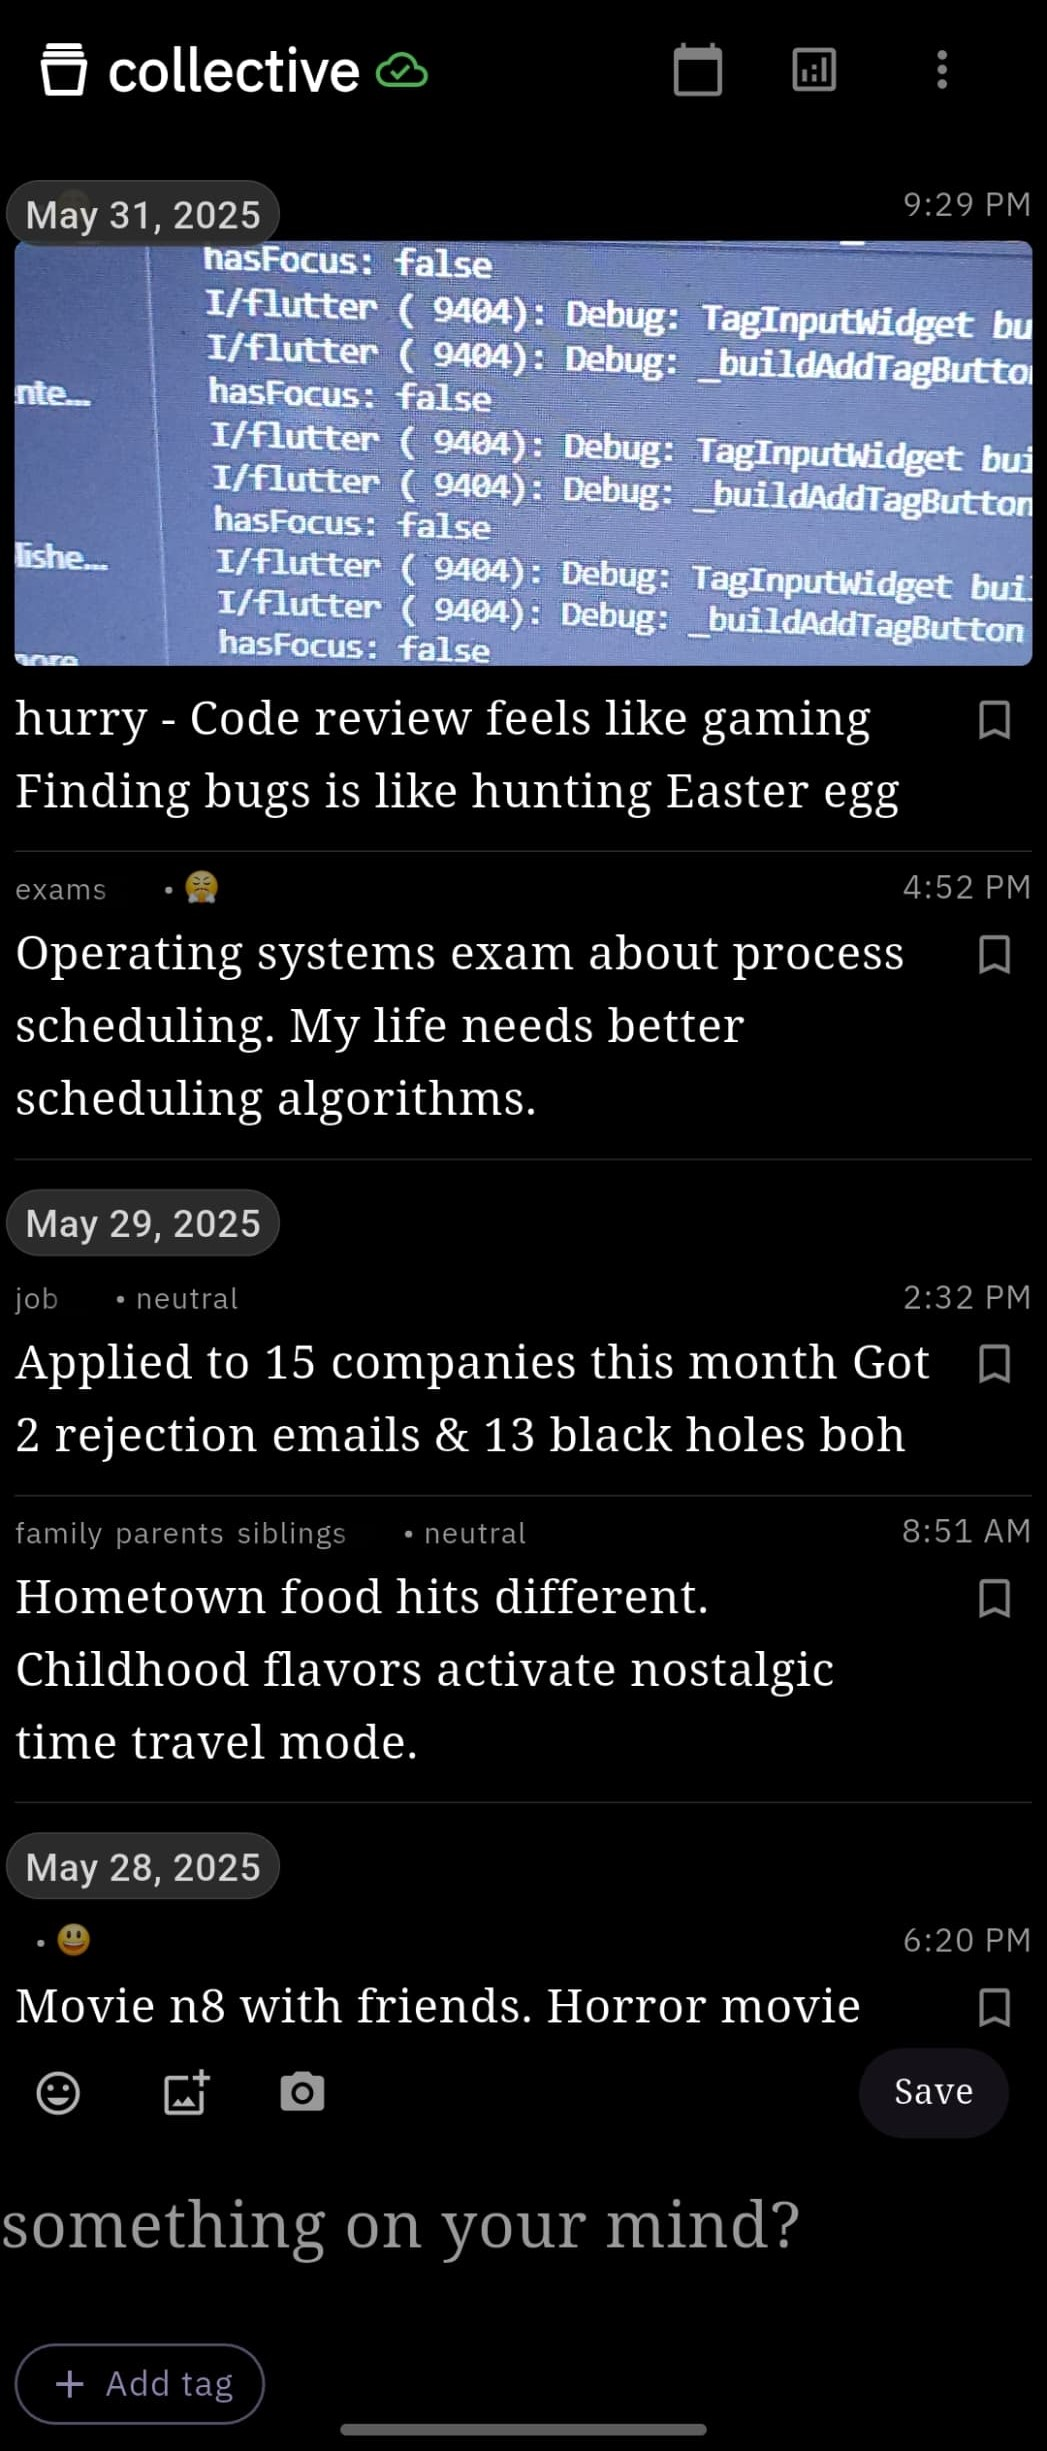
\includegraphics[width=0.4\textwidth]{files/imgs/prototype/journal_screen.jpeg}
\caption{Journal home screen showing entry timeline}
\label{fig:journal-screen}
\end{figure}
\end{samepage}

\subsubsection{Journal Input Interface}

The journal input interface emphasizes distraction-free writing with a minimalist text editor that expands as users type. The interface includes subtle features like mood selection through emoji picker, tag input with AI-powered suggestions, and multimedia attachment capabilities including camera integration for photos and GIF creation. The interface includes automatic saving to prevent data loss and provides visual feedback for all user actions.

\begin{samepage}
\begin{figure}[H]
\centering
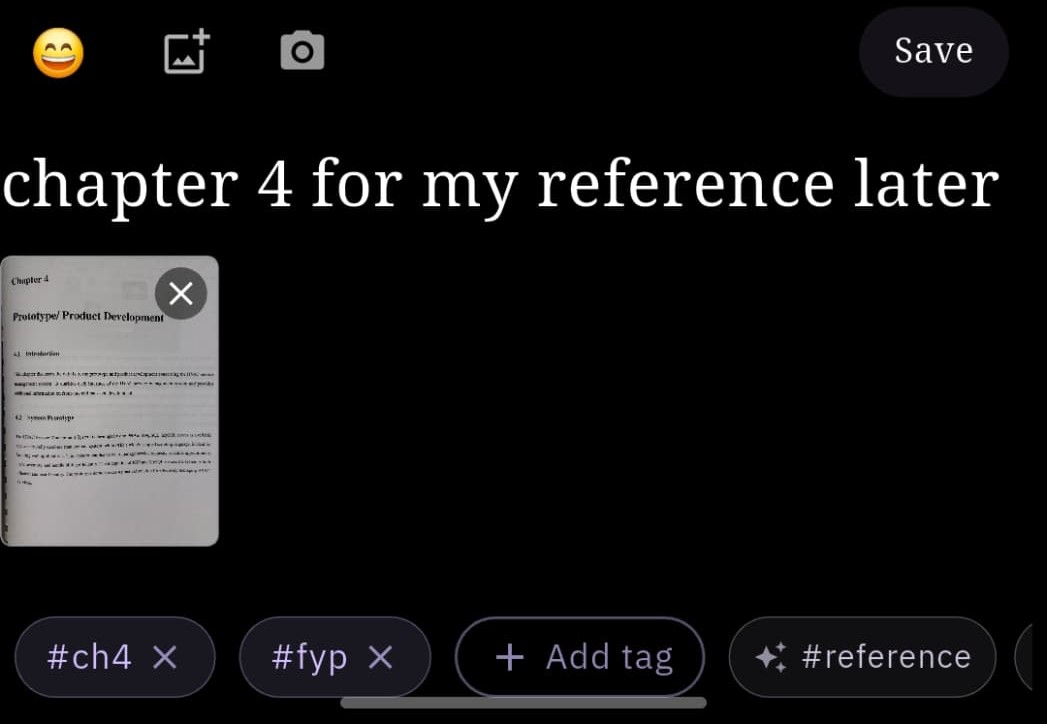
\includegraphics[width=0.4\textwidth]{files/imgs/prototype/journal_input_basic.jpeg}
\caption{Basic journal input interface for writing entries}
\label{fig:journal-input-basic}
\end{figure}
\end{samepage}

\paragraph{Emoji Selection Interface}

The emoji selection feature provides an expandable emoji bar for mood selection. Users can tap to reveal a collection of mood-representing emojis that help categorize their emotional state while writing. The emoji bar integrates seamlessly with the writing interface without disrupting the flow of composition.

\begin{figure}[H]
\centering
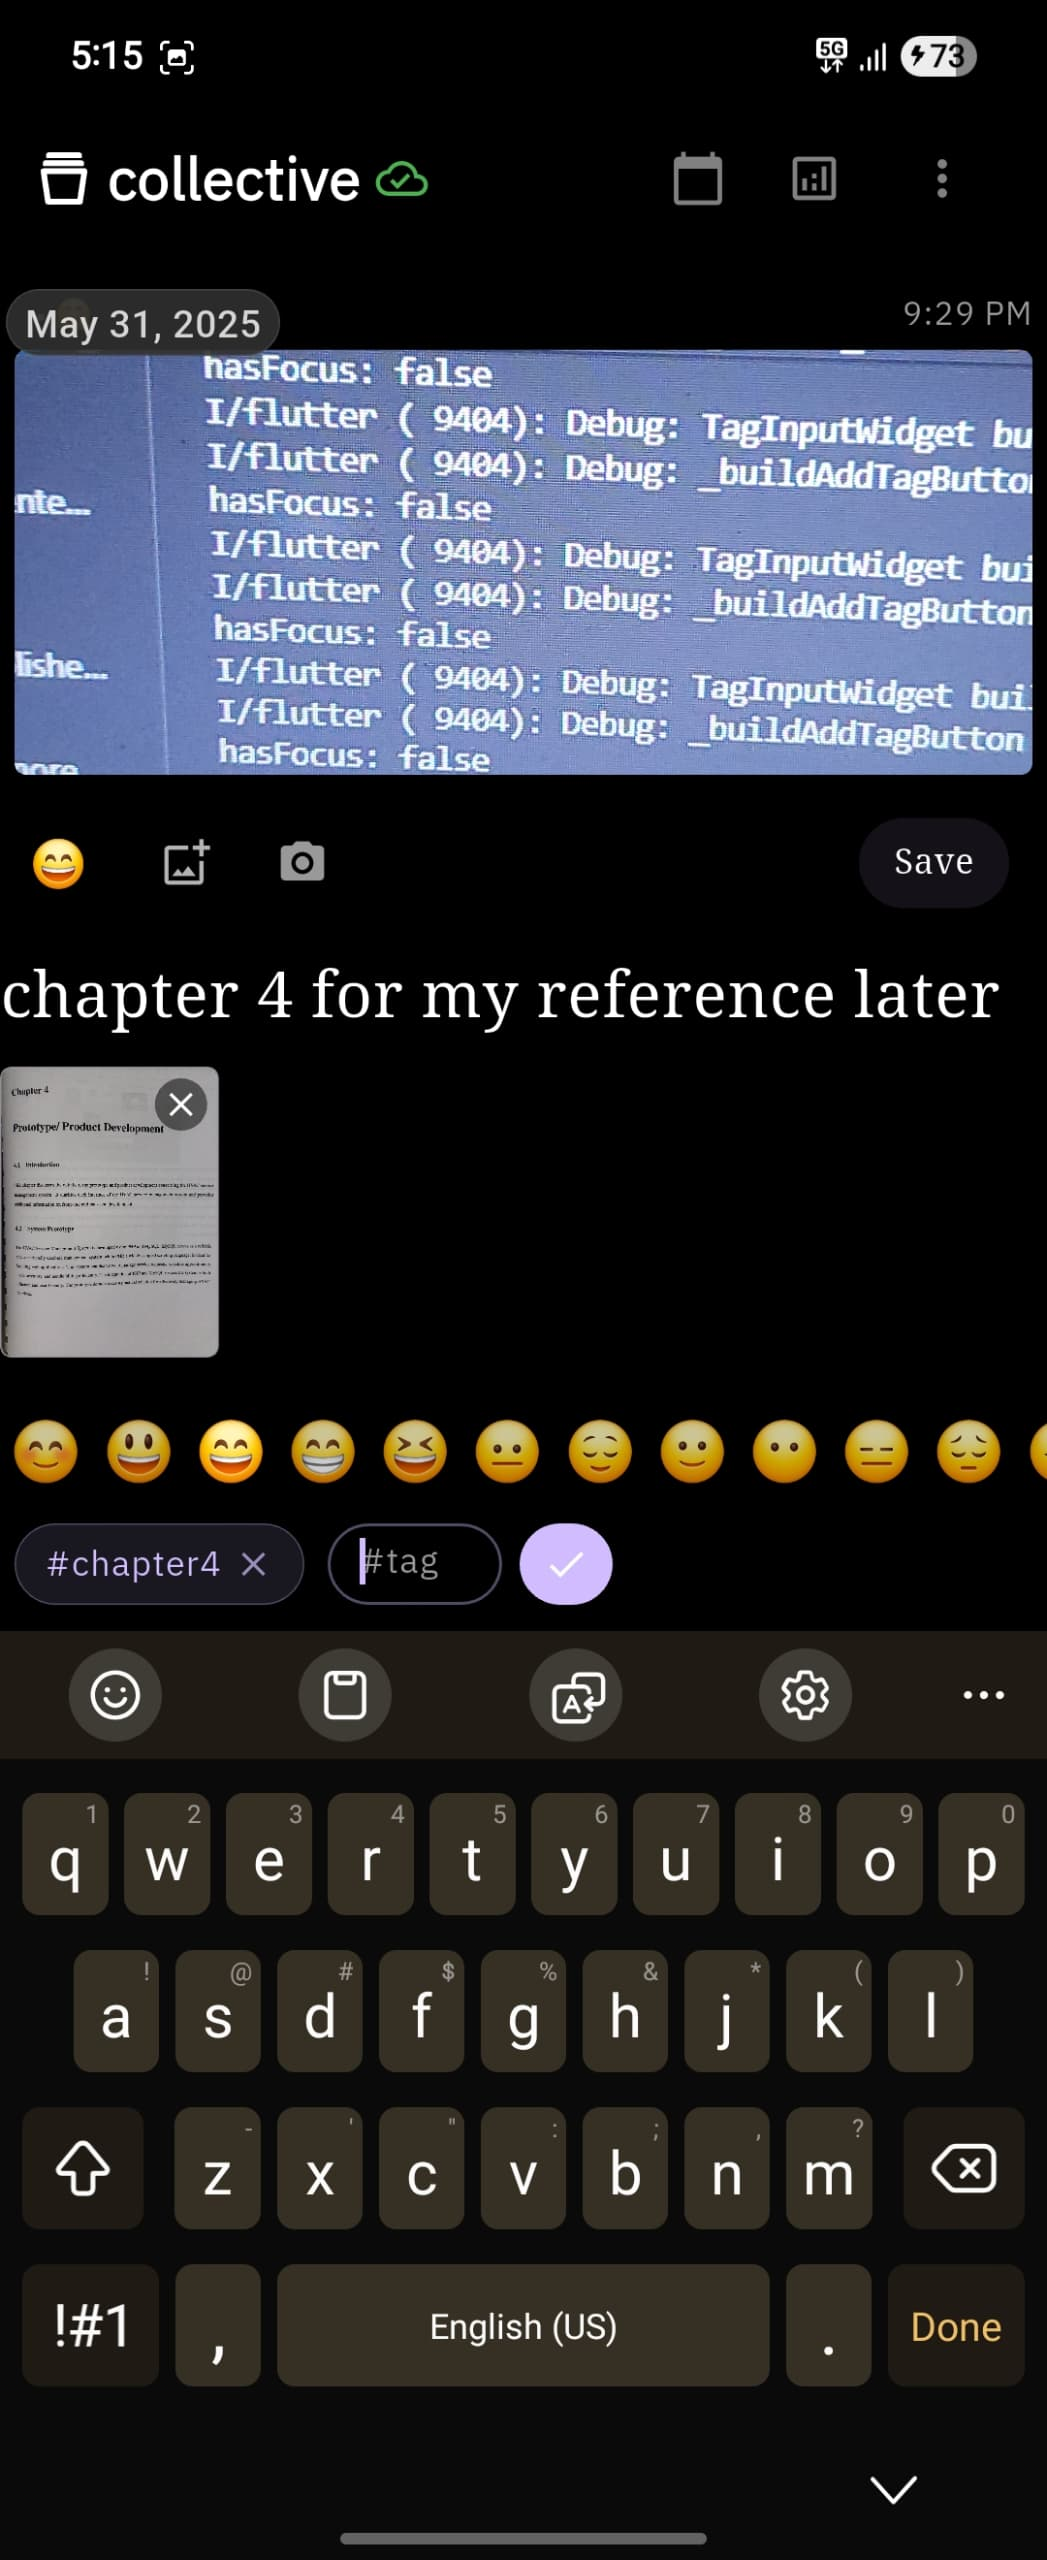
\includegraphics[width=0.4\textwidth]{files/imgs/prototype/emoji_selection.jpeg}
\caption{Emoji selection interface for mood indication}
\label{fig:emoji-selection}
\end{figure}

\paragraph{Photo Attachment Interface}

The photo attachment functionality allows users to add visual content to their journal entries. The interface provides options to select existing photos from the device gallery or capture new images using the camera. Photos are automatically compressed and optimized for storage while maintaining visual quality.

\begin{figure}[H]
\centering
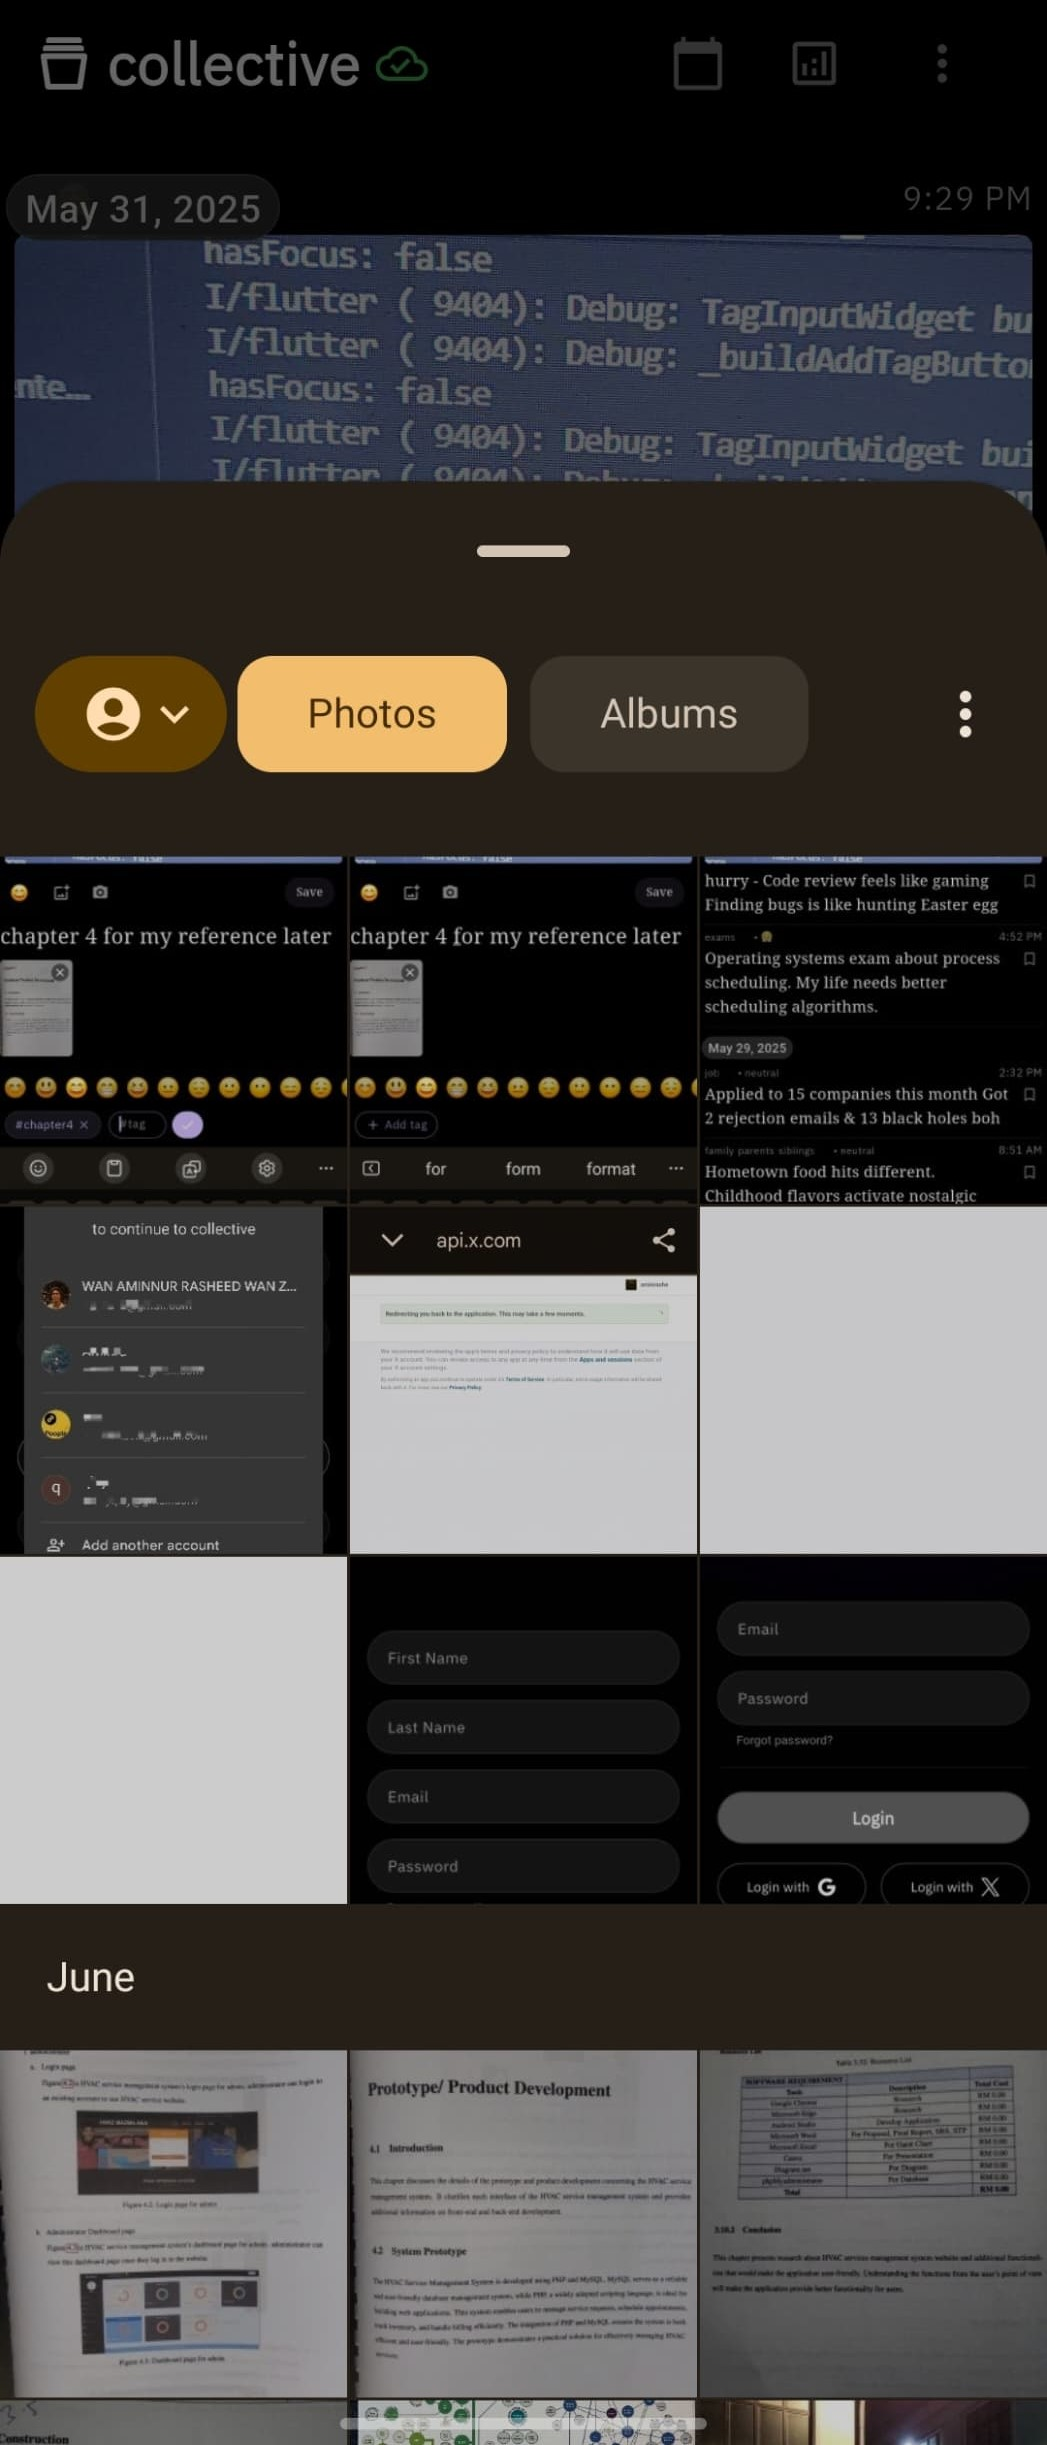
\includegraphics[width=0.4\textwidth]{files/imgs/prototype/photo_attachment.jpeg}
\caption{Photo attachment interface for adding images}
\label{fig:photo-attachment}
\end{figure}

\paragraph{Camera Integration}

The camera integration feature enables users to capture moments directly within the journal interface. The camera preview appears seamlessly within the app, allowing for immediate photo capture without leaving the writing context. The interface maintains focus on journaling while providing powerful multimedia capabilities.

\begin{figure}[H]
\centering
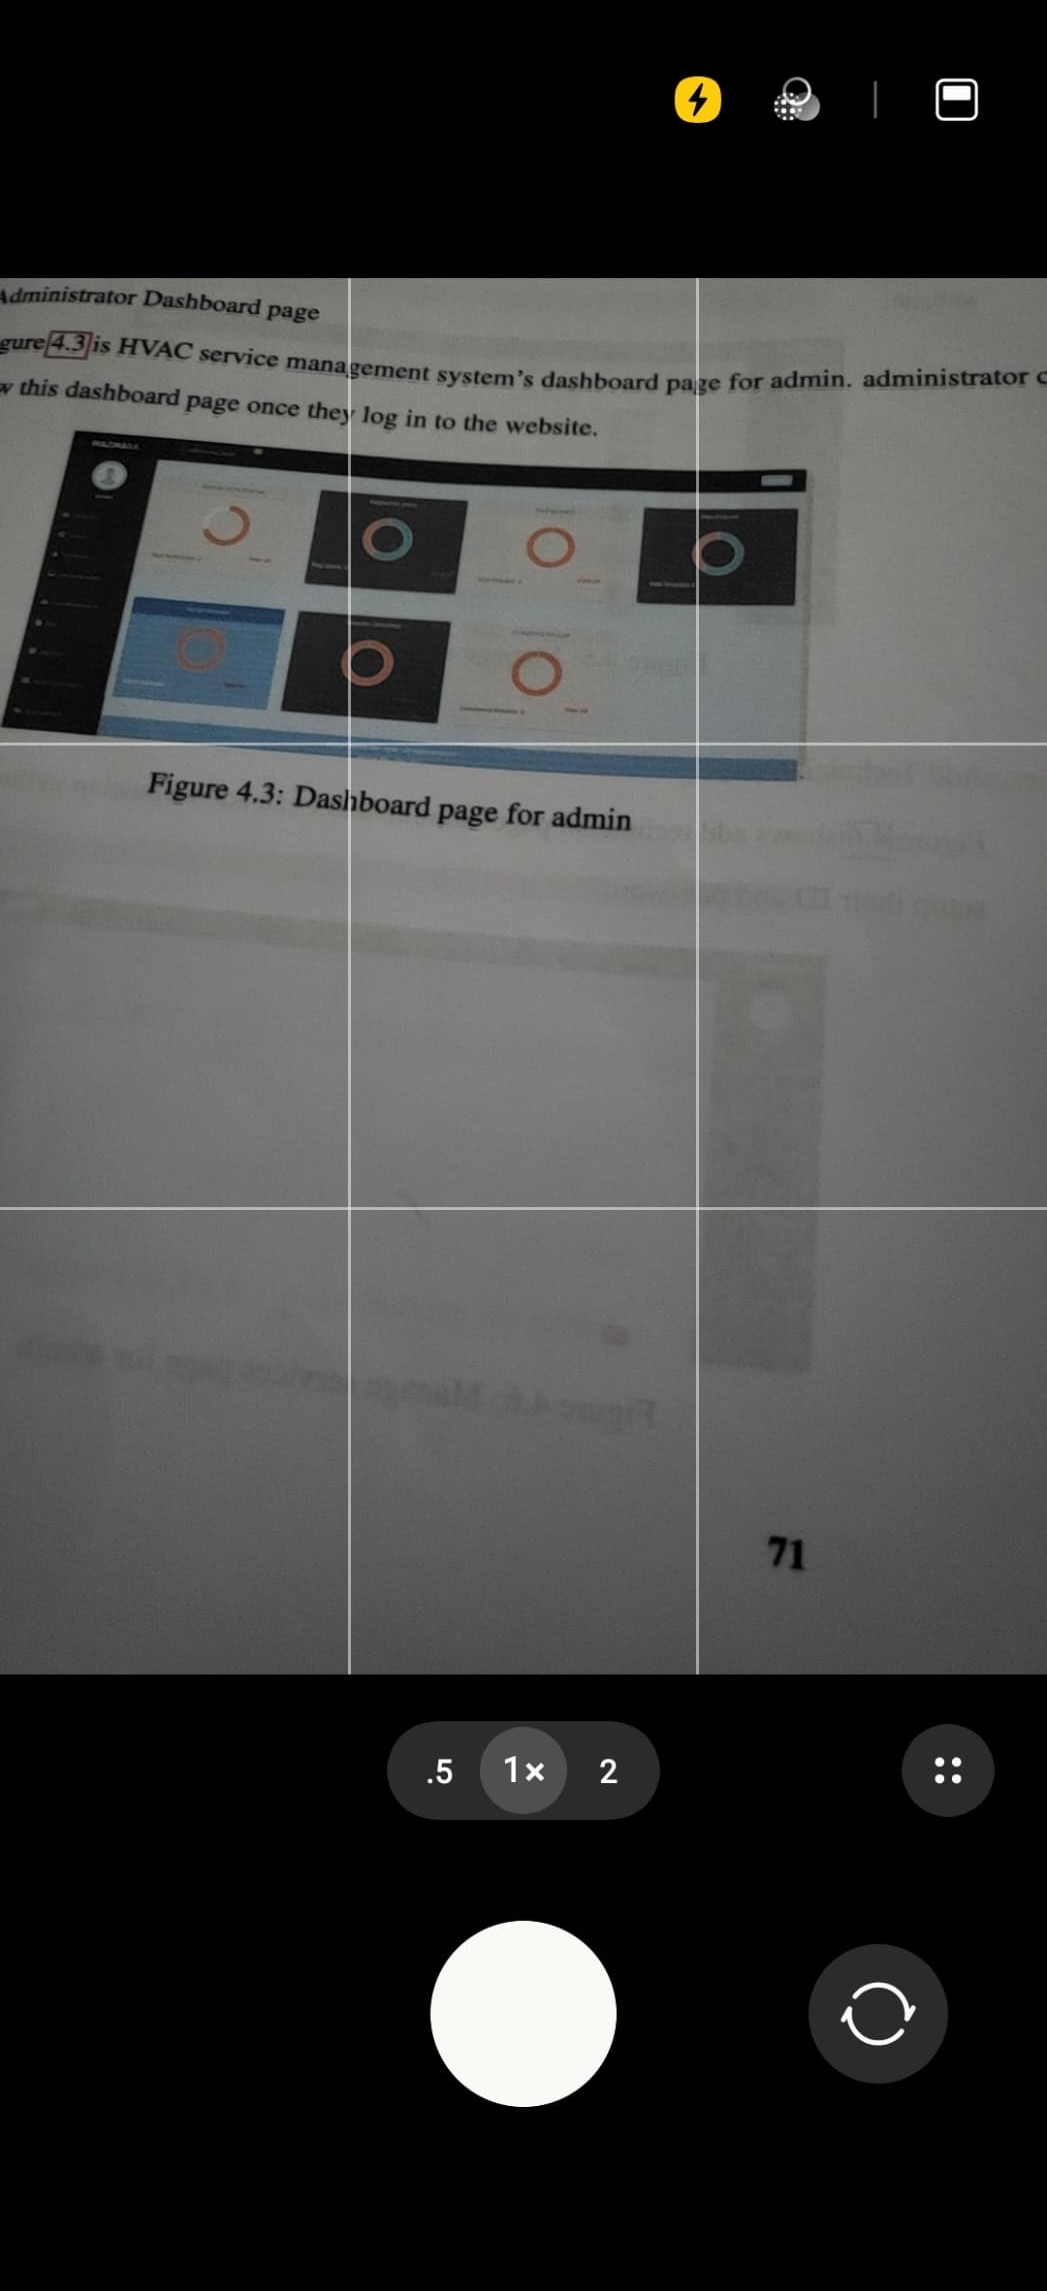
\includegraphics[width=0.4\textwidth]{files/imgs/prototype/camera_interface.jpeg}
\caption{Integrated camera interface for direct photo capture}
\label{fig:camera-interface}
\end{figure}

\paragraph{GIF Recording Functionality}

The GIF recording feature allows users to create short animated sequences to capture dynamic moments. Users can record brief video clips that are automatically converted to GIF format using FFmpeg processing. This feature adds a unique multimedia dimension to traditional journaling while maintaining storage efficiency.

\begin{figure}[H]
\centering
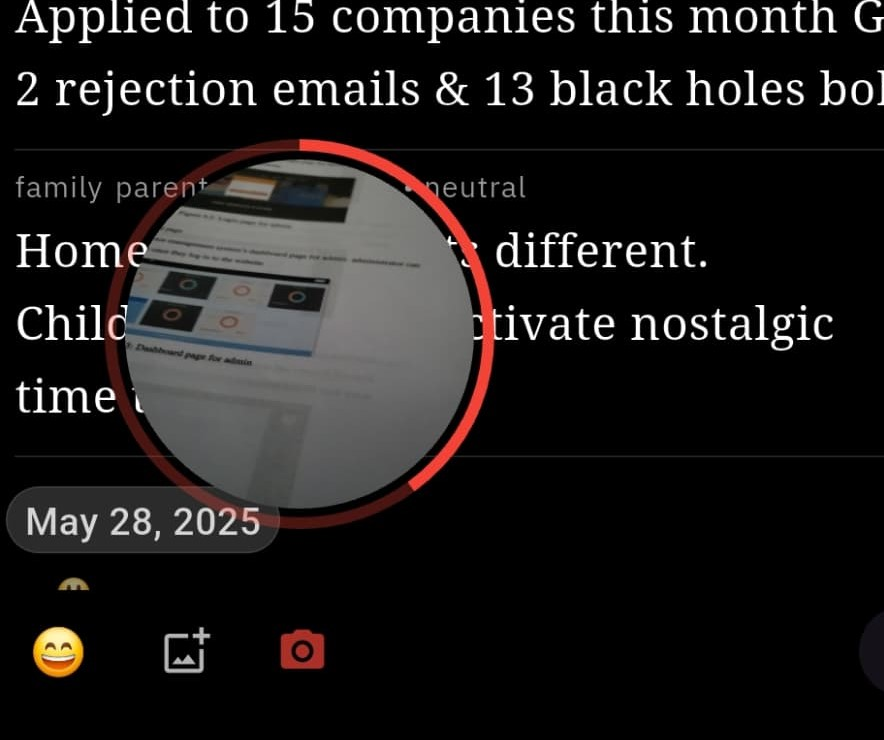
\includegraphics[width=0.4\textwidth]{files/imgs/prototype/gif_recording.jpeg}
\caption{GIF recording interface for creating animated content}
\label{fig:gif-recording}
\end{figure}

\paragraph{AI-Powered Tag Suggestions}

The tag suggestion system utilizes AI analysis to recommend relevant tags based on the entry content. As users type, the system analyzes the text in real-time and suggests contextually appropriate tags that help organize and categorize journal entries. The suggestions appear as subtle prompts that users can accept or ignore according to their preferences.

\begin{figure}[H]
\centering
\begin{minipage}{0.45\textwidth}
\centering

\includegraphics[width=0.9\textwidth]{files/imgs/prototype/tag_input.jpeg}
\caption{Tag input interface}
\label{fig:tag-input}
\end{minipage}
\hfill
%\begin{minipage}{0.45\textwidth}
%\centering
%\includegraphics[width=0.9\textwidth]{path/to/tag_suggestions.png}
%\caption{AI-powered tag suggestions}
%\label{fig:tag-suggestions}
%\end{minipage}
\end{figure}

\subsection{Navigation and Discovery}

\subsubsection{Search Functionality}

The search functionality enables users to quickly locate specific journal entries based on content, tags, mood, or date ranges. The search interface features a prominent search bar that supports both text-based queries and advanced filtering options. Users can search through their entire journal history with real-time results that highlight matching content within entries.

\begin{samepage}
\begin{figure}[H]
\centering
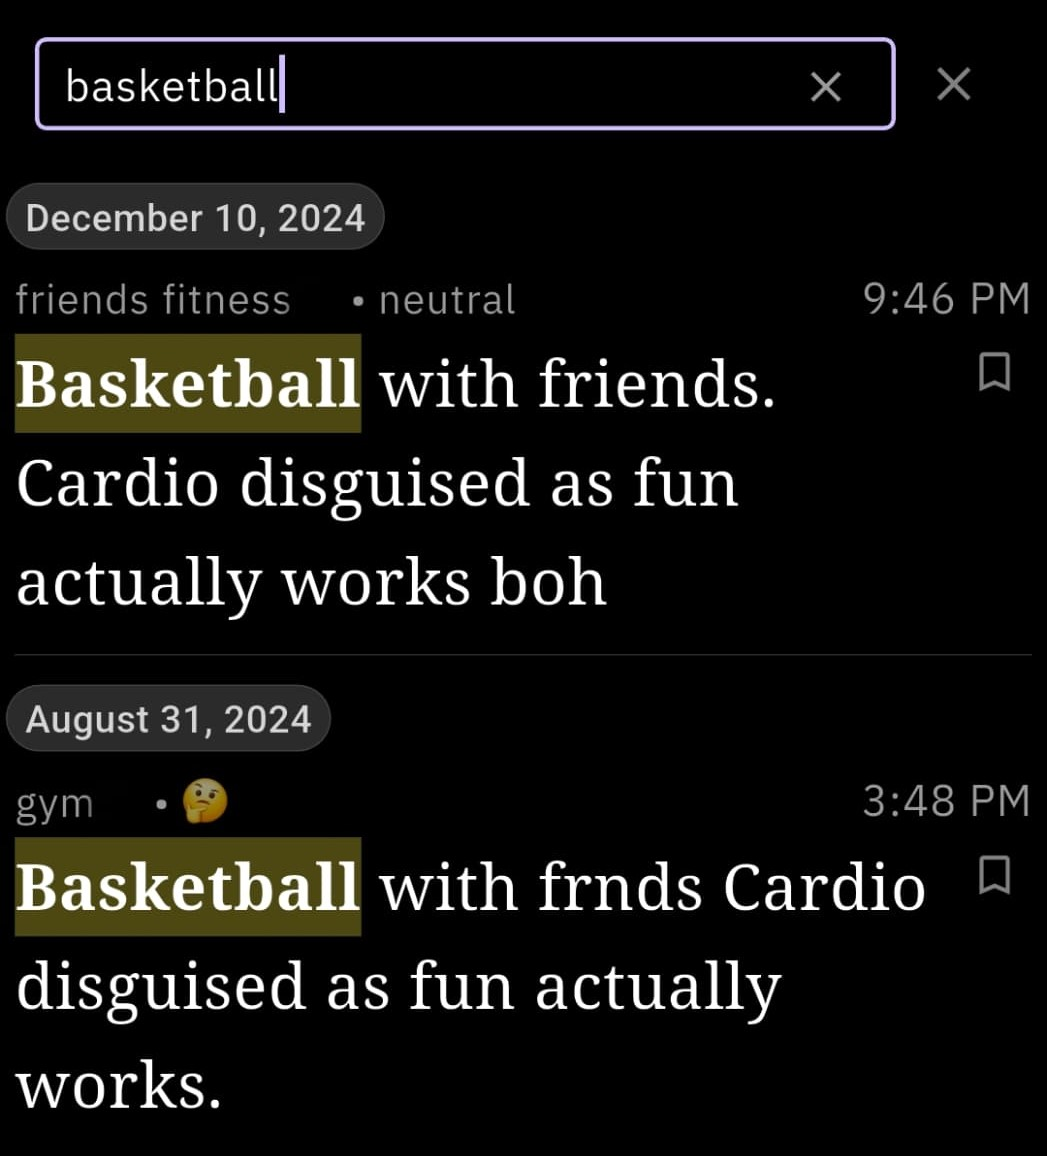
\includegraphics[width=0.4\textwidth]{files/imgs/prototype/search_interface.jpeg}
\caption{Search interface for finding journal entries}
\label{fig:search-interface}
\end{figure}
\end{samepage}

The search system implements intelligent filtering that considers entry content, associated tags, mood indicators, and temporal patterns. Results are displayed in a familiar timeline format with highlighted search terms, allowing users to quickly identify relevant entries and navigate to full content.

\subsubsection{Calendar Browsing Interface}

The calendar browsing feature provides a visual overview of journaling activity across time periods. Users can access a monthly calendar view that displays entry indicators for each day, allowing for quick navigation to specific dates and visual recognition of journaling patterns. The calendar interface integrates seamlessly with the main journal timeline.

\begin{samepage}
\begin{figure}[H]
\centering
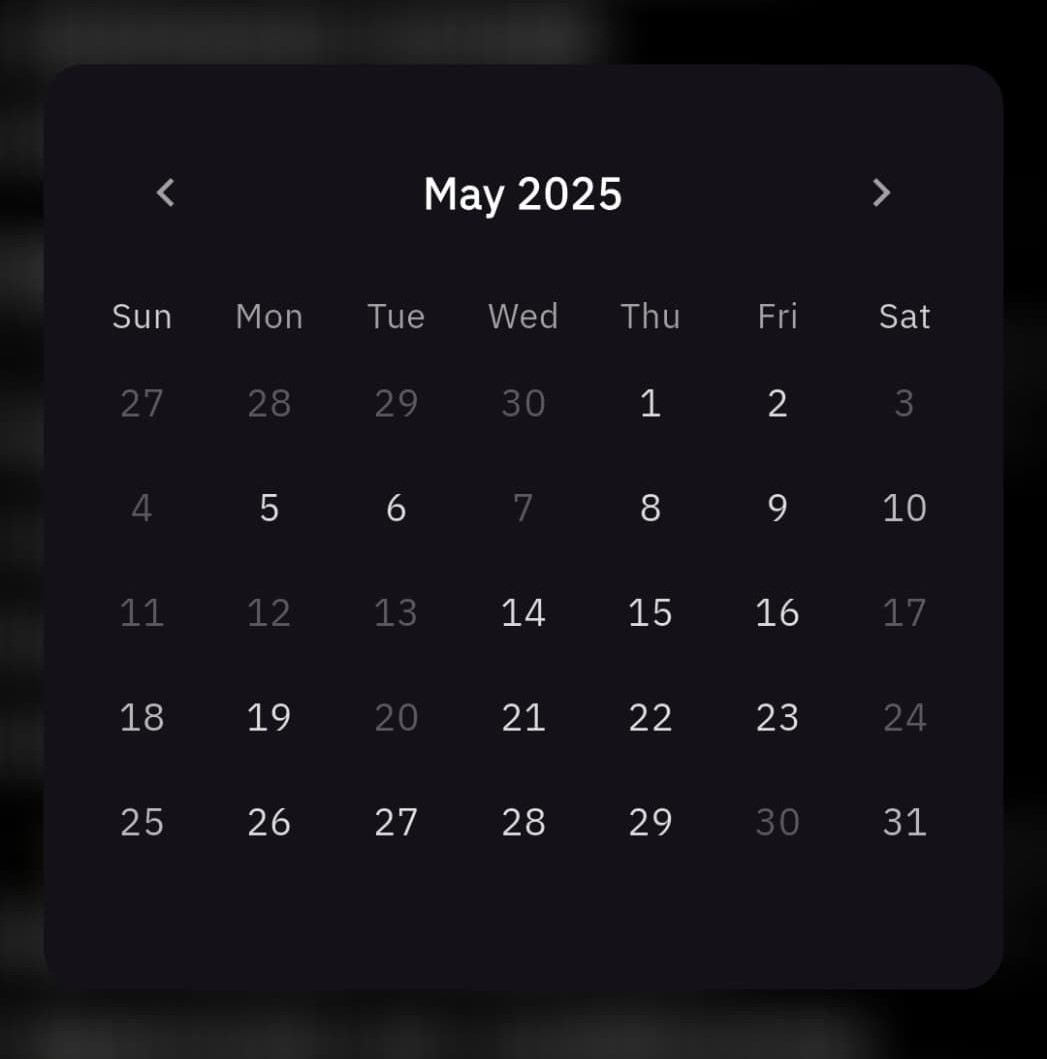
\includegraphics[width=0.4\textwidth]{files/imgs/prototype/calendar_browsing.jpeg}
\caption{Calendar browsing interface for date-based navigation}
\label{fig:calendar-browsing}
\end{figure}
\end{samepage}

The calendar view includes visual indicators for entry density, mood patterns, and special annotations. Users can tap on any date to navigate directly to entries from that day, providing an intuitive way to browse historical content and identify temporal patterns in their journaling habits.

\subsection{Entry Management}

\subsubsection{Entry Insight Screen}

The entry insight screen provides detailed analysis of individual journal entries using AI-powered insights from DeepSeek API. The screen displays the full entry content along with AI-generated insights that help users understand patterns in their writing and emotional state. Related entries are suggested based on content similarity and themes. The insights are presented in markdown format with smooth loading animations and caching for offline access. The screen includes navigation to related entries and maintains a history of viewed insights for quick reference.

\begin{samepage}
\begin{figure}[H]
\centering
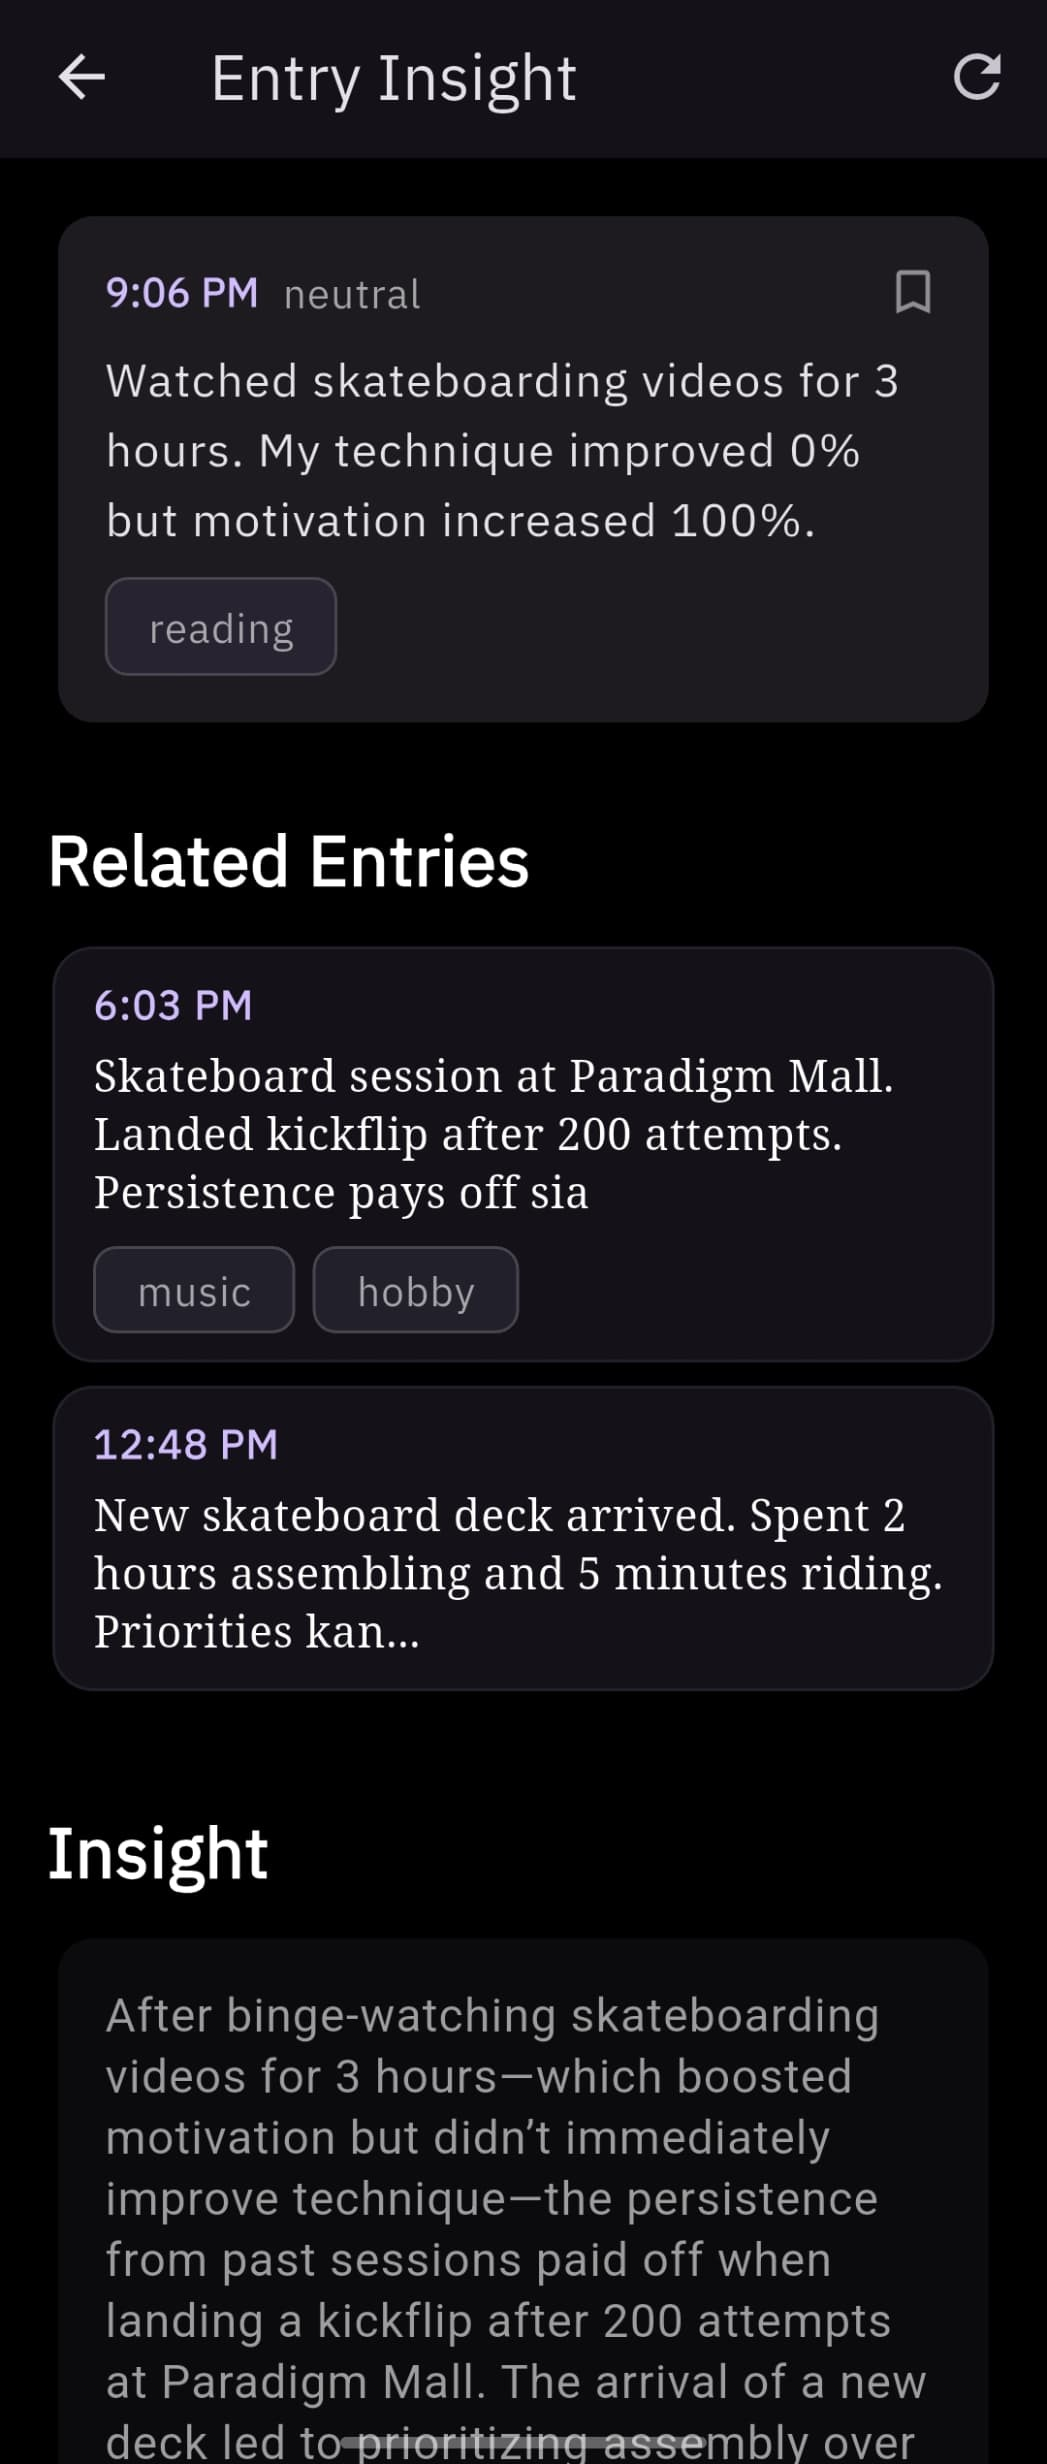
\includegraphics[width=0.4\textwidth]{files/imgs/prototype/entry_insight_screen.jpeg}
\caption{Entry insight screen with AI analysis}
\label{fig:entry-insight-screen}
\end{figure}
\end{samepage}

\subsubsection{Edit Entry Screen}

The edit entry screen allows users to modify existing journal entries while maintaining the original creation timestamp. The interface provides the same rich editing capabilities as the input widget, including mood modification, tag editing, and image management. Changes are tracked and saved automatically with visual feedback. The screen includes options to add or remove images, modify mood settings, and update tags. All changes are validated and synchronized with both local and cloud storage.

\begin{samepage}
\begin{figure}[H]
\centering
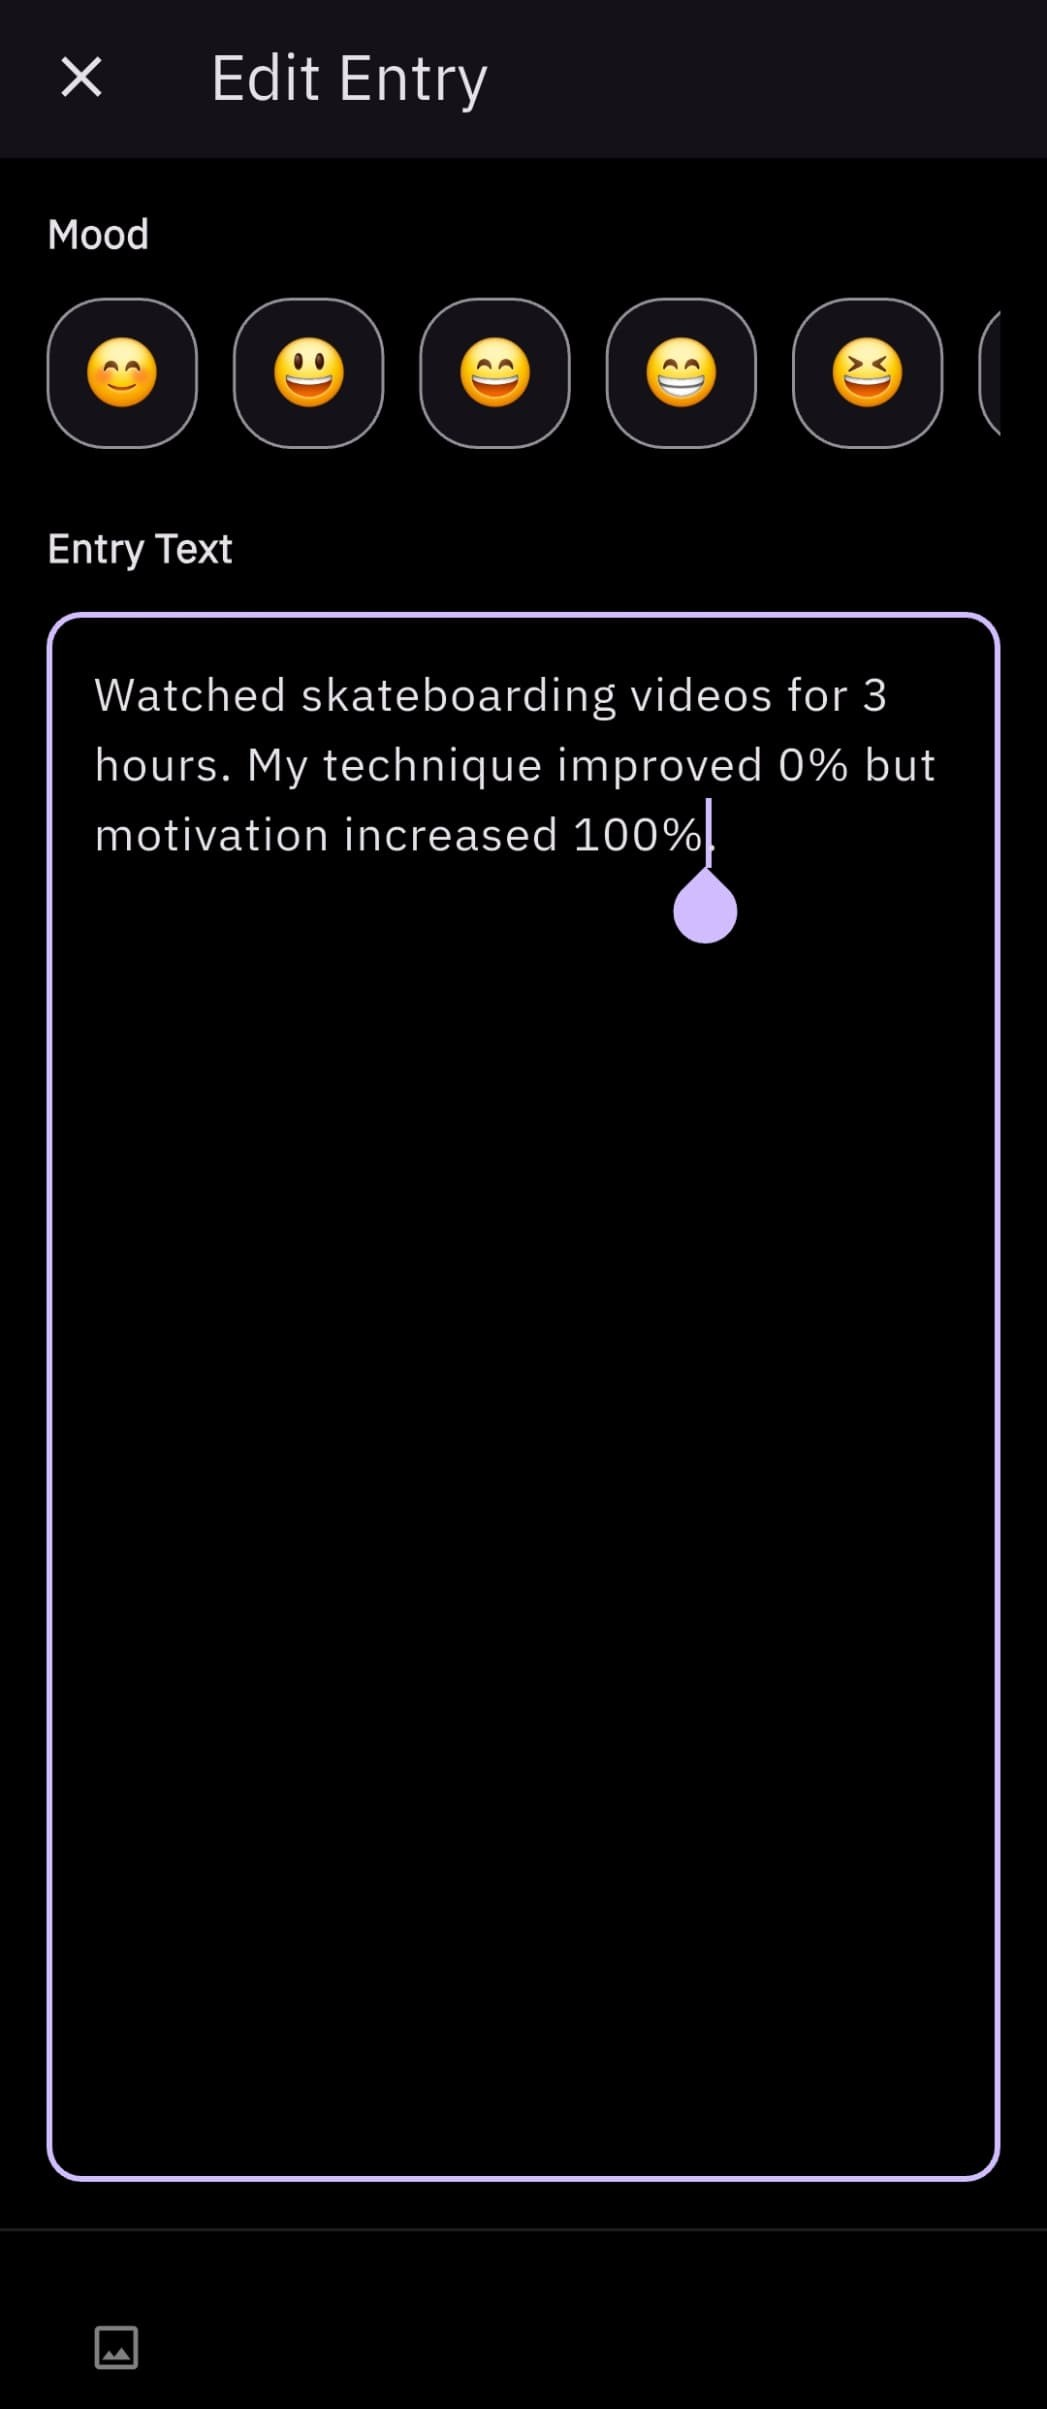
\includegraphics[width=0.4\textwidth]{files/imgs/prototype/edit_entry_screen.jpeg}
\caption{Edit entry screen for modifying entries}
\label{fig:edit-entry-screen}
\end{figure}
\end{samepage}

\subsection{Analytics and Insights}

\subsubsection{Analytics Dashboard}

The analytics screen presents comprehensive insights into journaling patterns and trends using visual representations of data. The interface includes calendar views showing journaling frequency, topic clustering analysis, and mood tracking over time. The analytics are generated using AI analysis of journal content while maintaining user privacy. Key features include topic clustering cards that group related entries, calendar heat maps showing writing frequency, and insights panels with AI-generated observations about writing patterns. The analytics cache intelligently to reduce processing time and API usage.

\begin{figure}[H]
\centering
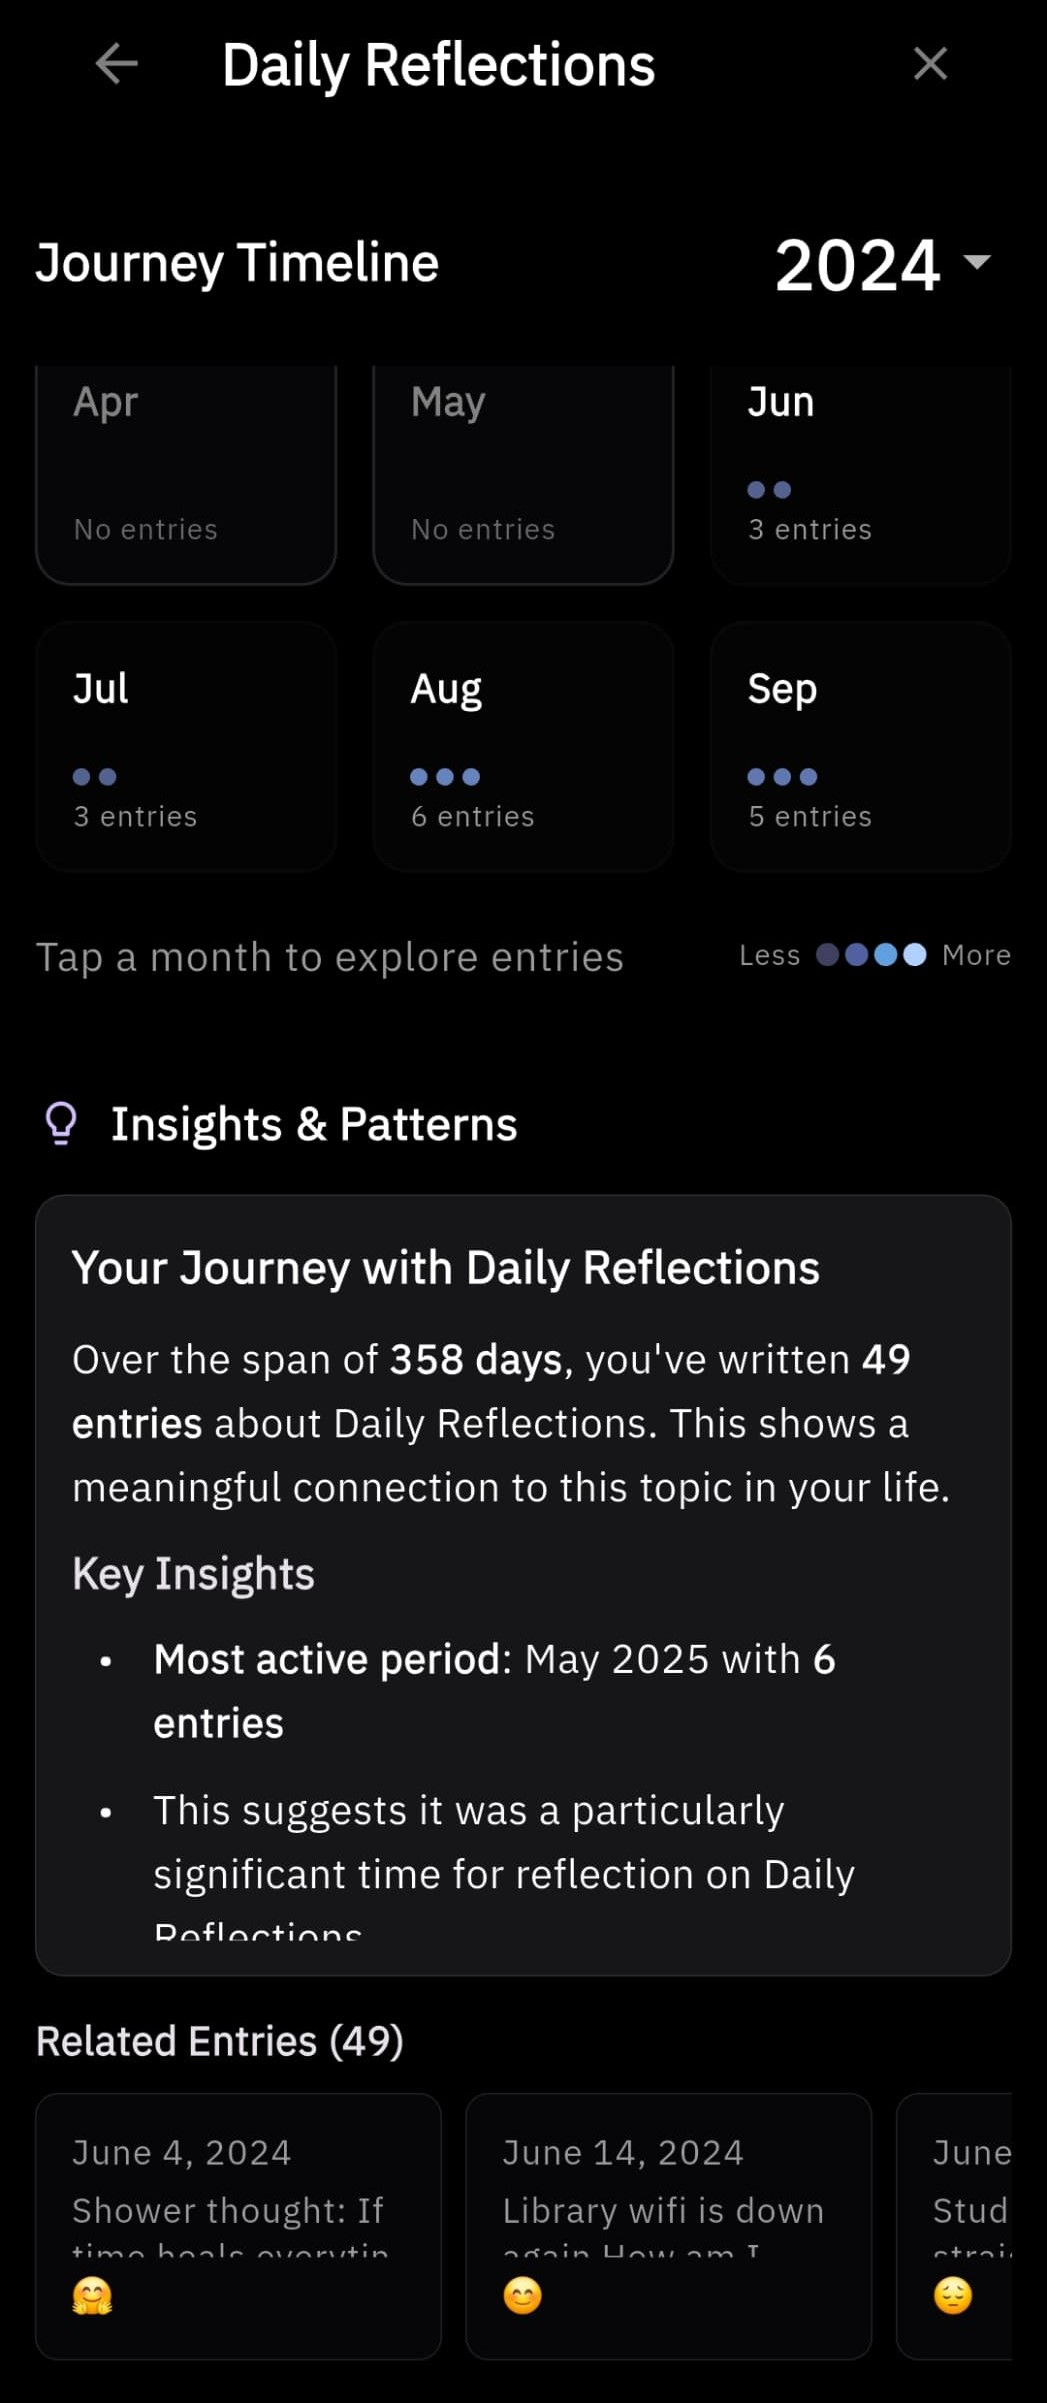
\includegraphics[width=0.4\textwidth]{files/imgs/prototype/analytics_screen.jpeg}
\caption{Analytics dashboard showing journaling patterns}
\label{fig:analytics-screen}
\end{figure}

\subsubsection{Topic Clustering Visualization}

The topic clustering feature automatically groups journal entries by themes and subjects using AI analysis. Each cluster is presented as a card showing the main topic, number of entries, and key themes. Users can explore clusters to find related content across different time periods.

\begin{figure}[H]
\centering
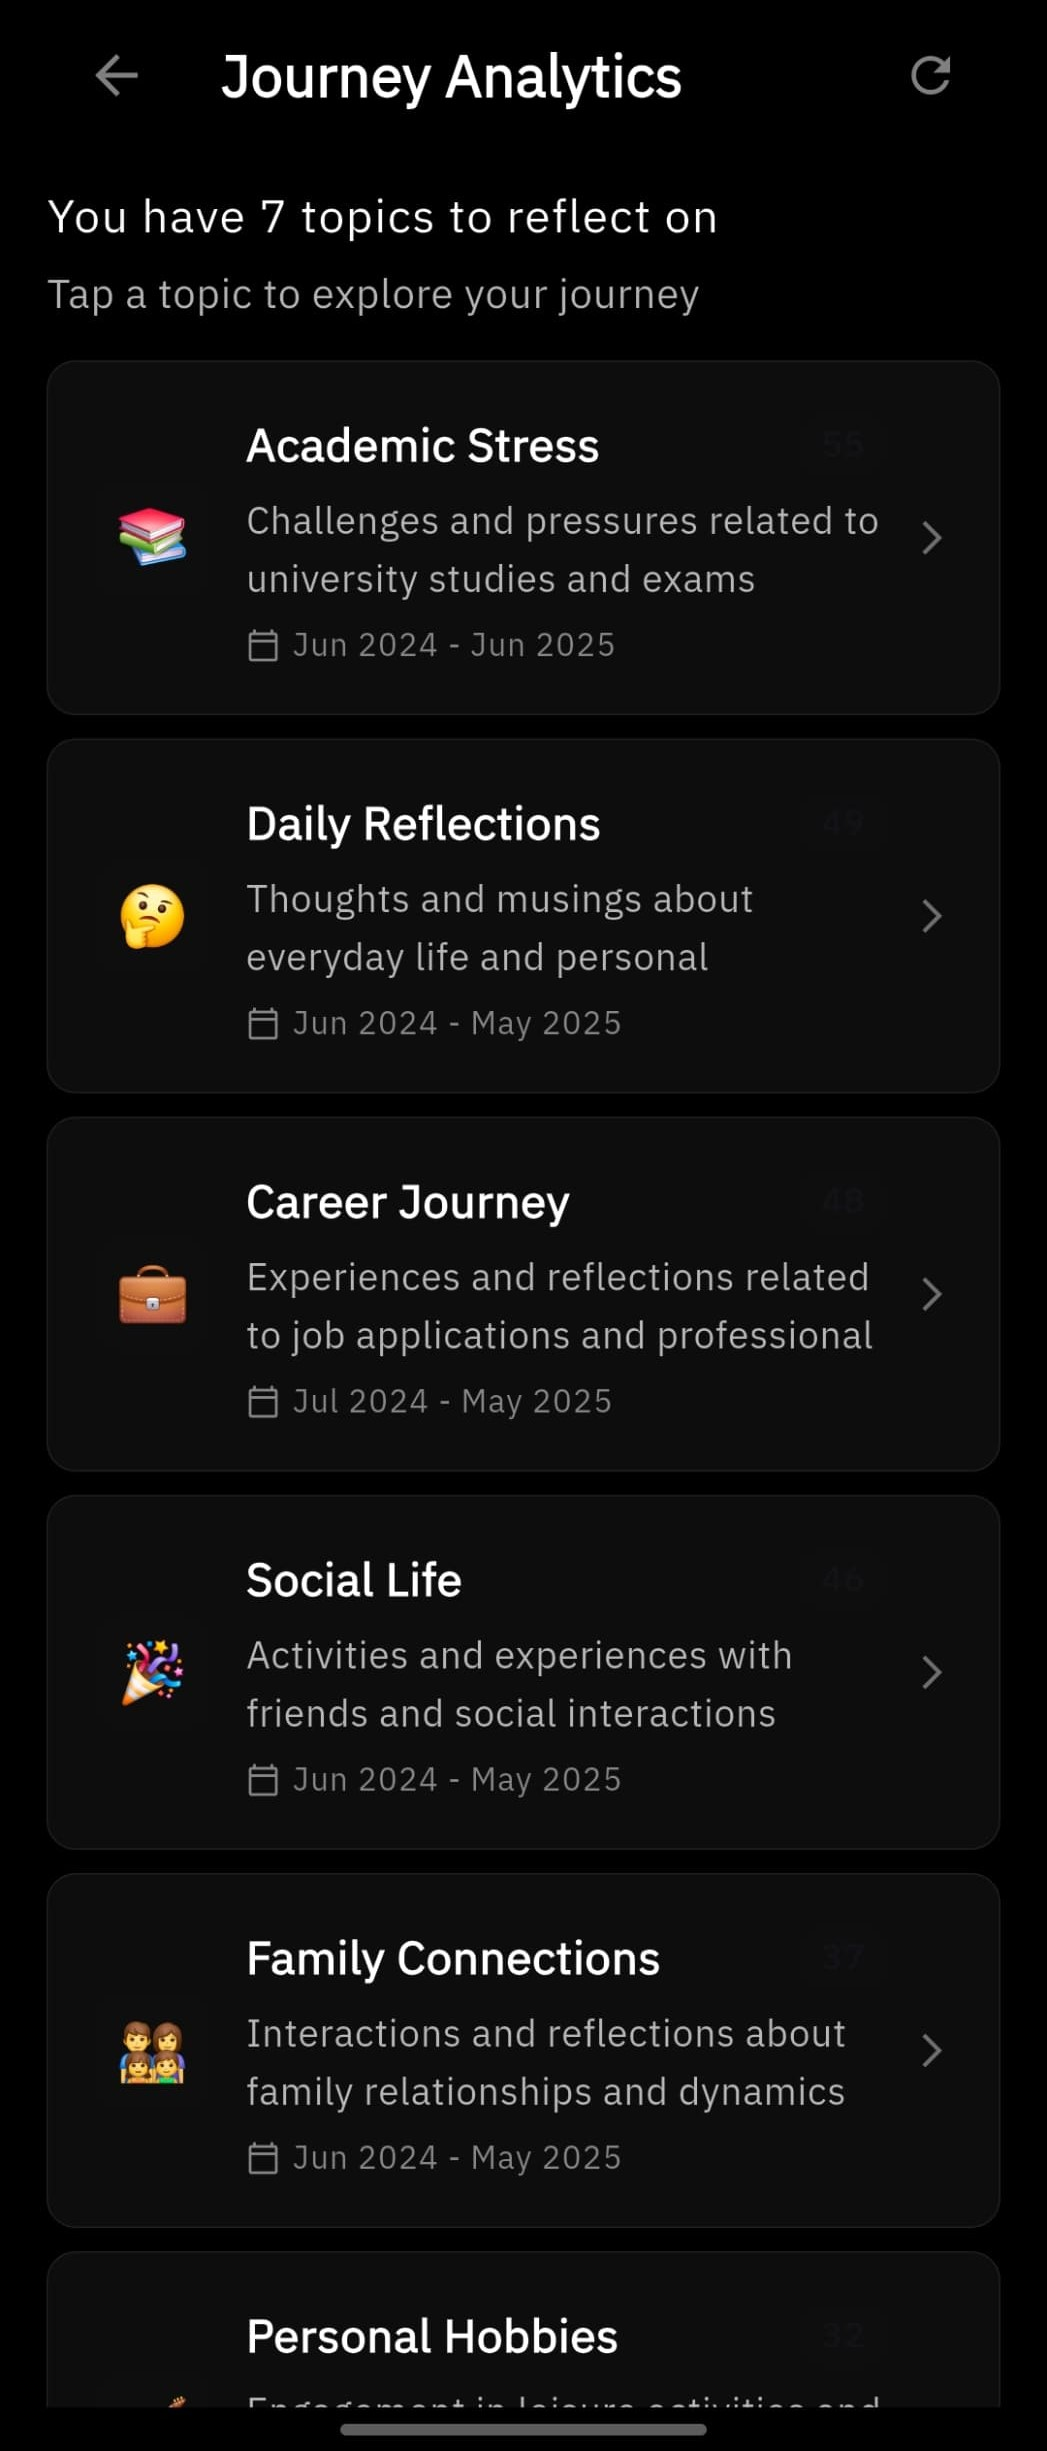
\includegraphics[width=0.4\textwidth]{files/imgs/prototype/topic_clustering.jpeg}
\caption{Topic clustering visualization}
\label{fig:topic-clustering}
\end{figure}

\subsection{Favorites and Collections}

\subsubsection{Favorites Screen}

The favorites screen displays a curated collection of entries that users have marked as favorites. The interface follows the same design patterns as the main journal screen but filters to show only favorited content. Entries maintain their original date grouping and include all standard interaction options. Users can easily unfavorite entries and access all entry details and insights from this screen. The interface provides quick access to frequently referenced content.

\begin{figure}[H]
\centering
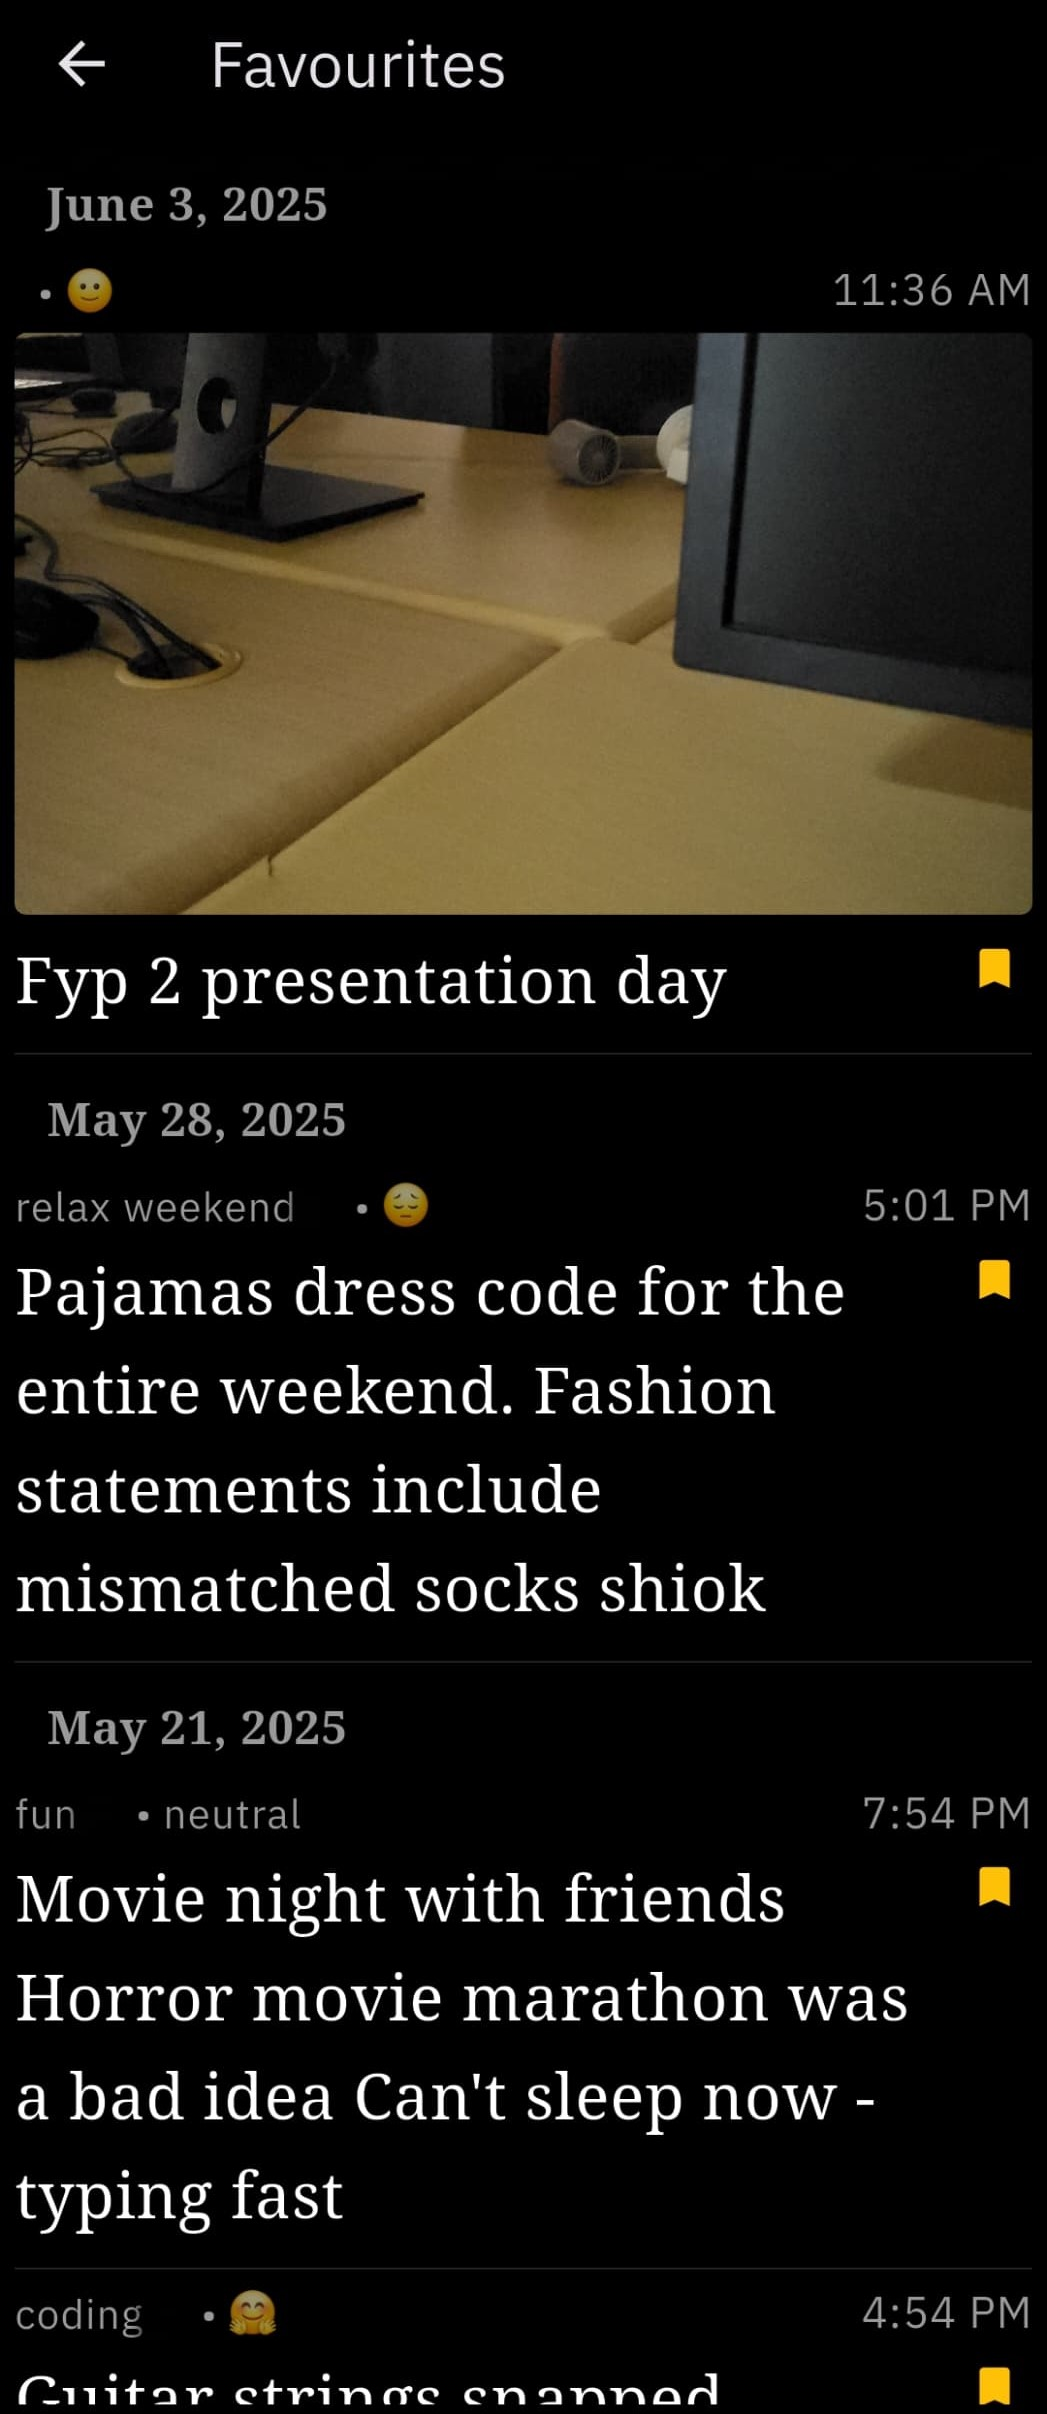
\includegraphics[width=0.4\textwidth]{files/imgs/prototype/favorites_screen.jpeg}
\caption{Favorites screen showing curated entries}
\label{fig:favorites-screen}
\end{figure}